\section{Euilerova metóda diskretizácie}
\label{se:diskretizacia}
Táto metóda je stará už vyše 200 rokov, ale aj napriek tomu sa používa dodnes. Je založená na numerickej diskretizácii. Chyba, ktorej sa dopúšťame použitím tejto metódy, je priamo úmerná kroku diskretizácie, ktorý zvolíme. Nie je až taká účinná v porovnaní s ostatnými metódami, ale je používaná ako základ komplexnejších metód. Pre účely nášho projektu bude postačujúca v základnej forme a jej jednoduchosť bude pre nás výhodou.

Euilerová metóda má nasledovný matematický zápis
\begin{align}
	\dot{x}(t) &= f(x,t)\\
	x_{k+1} &= x_{k} + hf(x_{k})
\end{align}
kde h predstavuje dĺžku kroku, v našom projekte bude rovnaká, ako perióda vzorkovania diskretizovaného systému.
\begin{figure}[H]
	\centering
	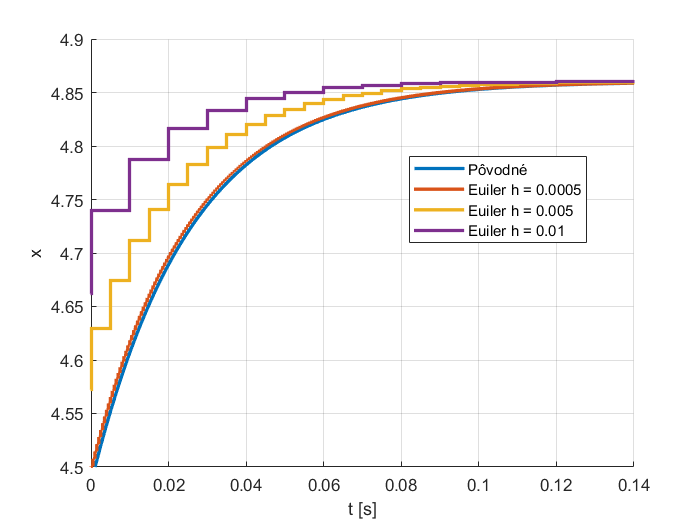
\includegraphics[width=11cm,height=8cm]{images/Euler_method}
	\caption{Eulierová diskretizácia}
\end{figure}
Ako môžeme vidieť na (Obr. 2.2), čím budeme používať menšiu periódu, tým presnejšia bude diskretizácia.

